\documentclass[10pt]{article}
\usepackage[a4paper,left=15mm,right=15mm,top=16mm,bottom=16mm]{geometry}
\usepackage{fontspec,graphicx,xcolor}
\setmainfont{Arial}
\setsansfont{Arial}
\pagestyle{empty}
\setlength{\parindent}{0pt}
\setlength{\parskip}{0pt}
\setlength{\emergencystretch}{1em}
\begin{document}
{\fontsize{13}{16}\selectfont\bfseries Figure 1}\par\vspace{3mm}
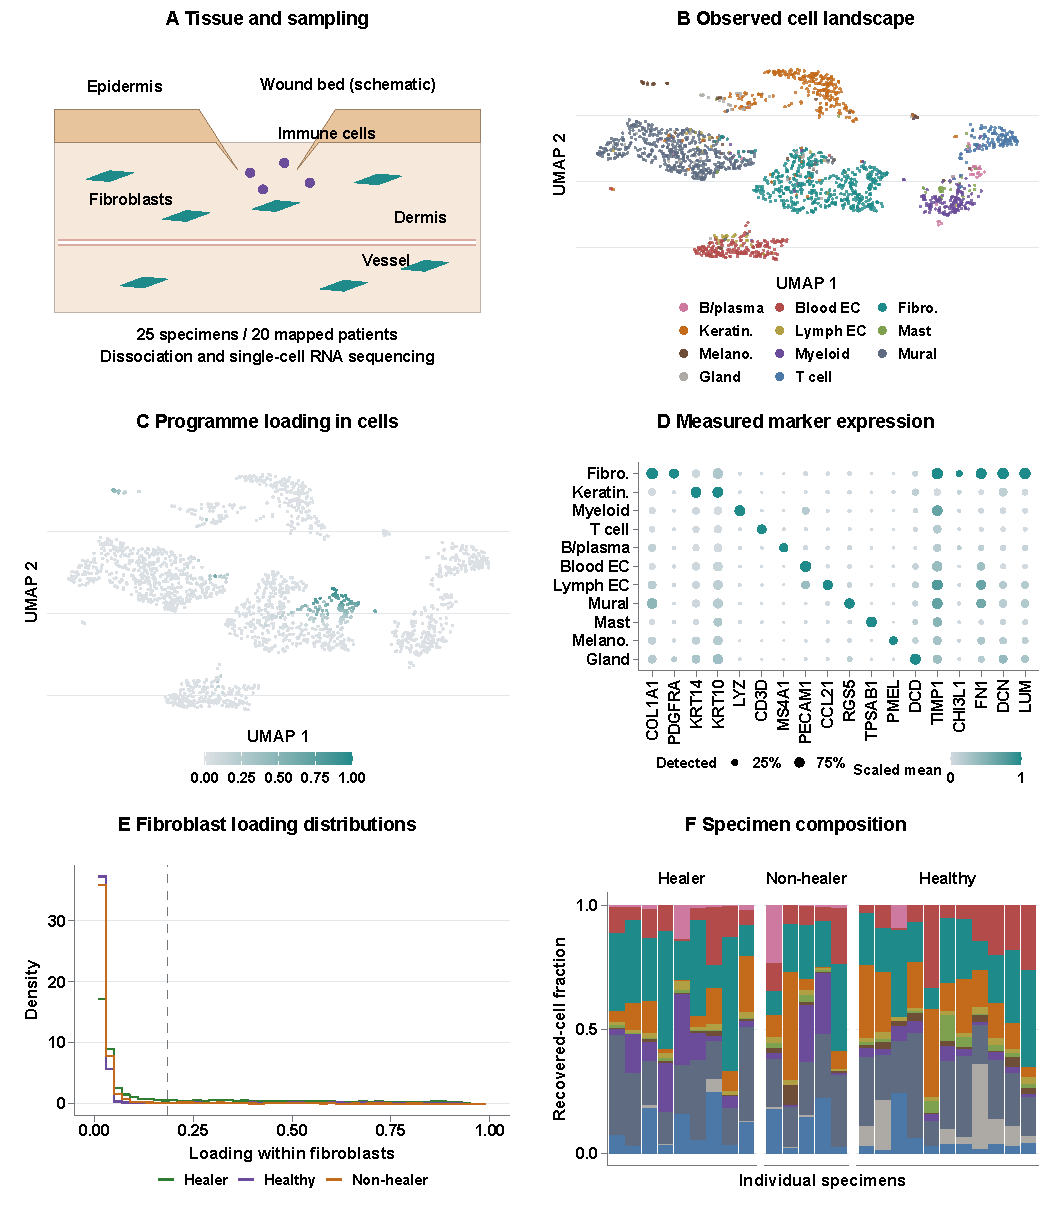
\includegraphics[width=180mm]{../figure1_workflow.pdf}\par\vspace{3mm}
{\fontsize{9}{11.5}\selectfont Foot-skin material, model readouts and expression context. (A) Conceptual tissue, not histology: 9 healing specimens from 7 patients, 5 non-healing specimens from 4 patients, and 11 non-diabetic specimens from 9 patients. Frozen inference maps 7,002-gene proportions through the Gaussian-encoder mean μ and 15-topic softmax θ to two separate readouts: marker-gated fibroblast mean/fraction and the all-cell patient mean used for the primary outcome contrast. Neither readout feeds the other. The separate training route samples Gaussian z and reconstructs proportions through softmax(z) and normalized decoder β, with cross-entropy plus 0.01 Gaussian KL. (B) A uniform 2,000-cell display subset of 76,461 cells, colored by marker-derived lineage on UMAP. Fibro., fibroblast; EC, endothelial cell; mural, pericyte/smooth muscle. (C) The same cells colored by continuous frozen loading, not new cell types. (D) Measured expression in all retained cells: dot size is detection fraction, color gene-wise scaled mean log-normalized expression. Annotation markers do not independently validate the labels. (E) Fixed-bin histogram densities of all 19,410 fibroblast loadings, with the original threshold; non-diabetic patients lack healing outcomes. (F) Recovered-cell composition in 25 specimens, including repeated patients; colors match B. Inference uses full data and patient units, not the display subset.\par}
\newpage
{\fontsize{13}{16}\selectfont\bfseries Figure 2}\par\vspace{3mm}
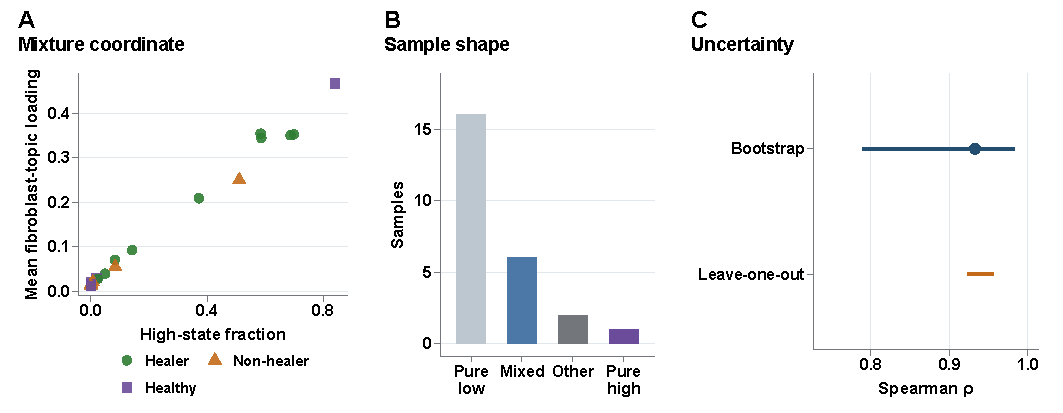
\includegraphics[width=180mm]{../figure2_mixture_semantics.pdf}\par\vspace{3mm}
{\fontsize{9}{11.5}\selectfont Association between mean topic loading within fibroblasts and the high-state fraction. (A) Each point is one of 25 GSE165816 specimens: 9 healing (green circles), 5 non-healing (orange triangles) and 11 healthy non-diabetic (purple squares). The high-state fraction uses the pooled cut 0.1842958; Spearman ρ=0.933. (B) Sample-shape counts use within-sample loading quantiles: pure low requires the 90th percentile at most 0.15, pure high the 10th percentile at least 0.10, and mixed the 10th percentile at most 0.05 and 90th percentile at least 0.40; other samples form the remaining category. (C) Unlike the specimen-level panels A and B, uncertainty uses 20 author-mapped patients after pooling repeated specimens by fibroblast count. The dot is the patient correlation 0.937, the blue segment is the descriptive 10,000-draw patient-bootstrap 95\% interval (0.776--0.990), and the orange segment is the leave-one-patient-out range (0.927--0.964). Both correlated summaries use the same cells; the association does not by itself prove stable within-state intensity or a healing effect.\par}
\newpage
{\fontsize{13}{16}\selectfont\bfseries Figure 3}\par\vspace{3mm}
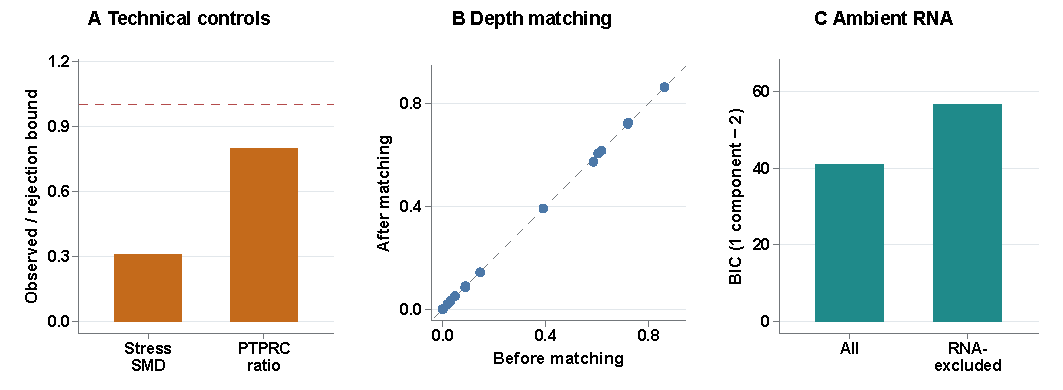
\includegraphics[width=180mm]{../figure3_artifact_controls.pdf}\par\vspace{3mm}
{\fontsize{9}{11.5}\selectfont Technical and immune-transcript exclusion controls in the discovery cohort. (A) Dissociation standardized mean difference (SMD, 0.246) and the high-state/low-state PTPRC-positive rate ratio (1.60) are divided by rejection bounds 0.8 and 2.0; the dashed line is one. The rounded state cut is 0.184. (B) Each point is one of 25 samples after restricting to 14,561 fibroblasts eligible for panel-count matching to 986 counts per cell. Reprojection preserves sample fractions (ρ=0.984) and 99.5\% of cell labels; the dashed line is identity. (C) Bars are BIC for one Gaussian minus BIC for two Gaussians fitted to sample high-state fractions, using 24 matched samples before and after exclusion. Positive values favour two components. Exclusion retains 11,262 of 19,410 fibroblasts overall, and matched sample fractions correlate at ρ=0.989. This control measures invariance to the exclusion rule; it does not identify every source of ambient RNA or tissue-composition dependence.\par}
\newpage
{\fontsize{13}{16}\selectfont\bfseries Figure 4}\par\vspace{3mm}
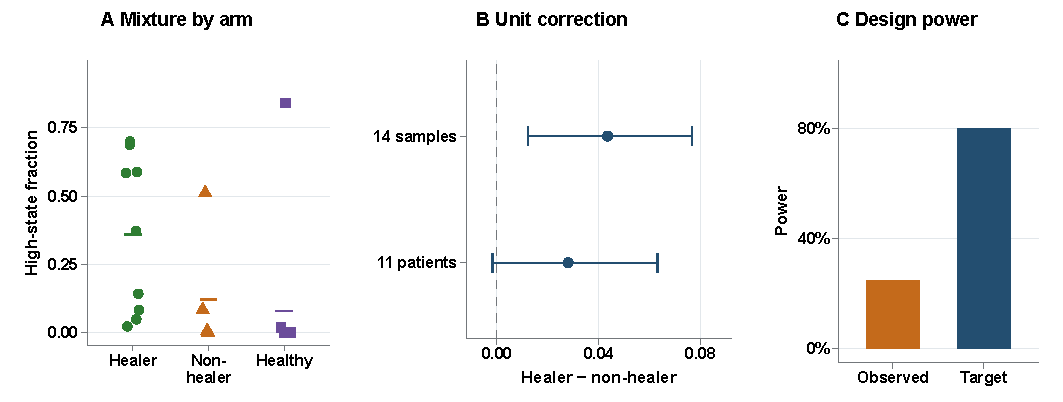
\includegraphics[width=180mm]{../figure4_outcome_counterexample.pdf}\par\vspace{3mm}
{\fontsize{9}{11.5}\selectfont State abundance, analysis unit and design power. (A) Symbols show high-state fractions for 9 healing, 5 non-healing and 11 healthy specimens; horizontal segments mark arm means. Green circles, orange triangles and purple squares identify these groups. The largest fraction is 0.841 in healthy non-diabetic foot skin, showing that the state is not exclusive to healing ulcers. (B) Dots and within-arm bootstrap 95\% intervals show the healing-minus-non-healing difference in all-cell mean fibroblast-associated topic loading for 14 specimens and 11 mapped patients. The patient analysis resamples 7 healing and 4 non-healing patients in 30,000 draws. Its readout differs from the fibroblast high-state fraction in A; the vertical dashed line is zero. (C) Gaussian location-shift simulation with a two-sided Mann--Whitney test estimates 24.9\% power for the separate 9-versus-5 high-state-fraction design, against an 80\% target. Its minimum detectable difference is 0.519. These are design sensitivities, not effect-exclusion bounds or clinical minimum important differences.\par}
\newpage
{\fontsize{13}{16}\selectfont\bfseries Figure 5}\par\vspace{3mm}
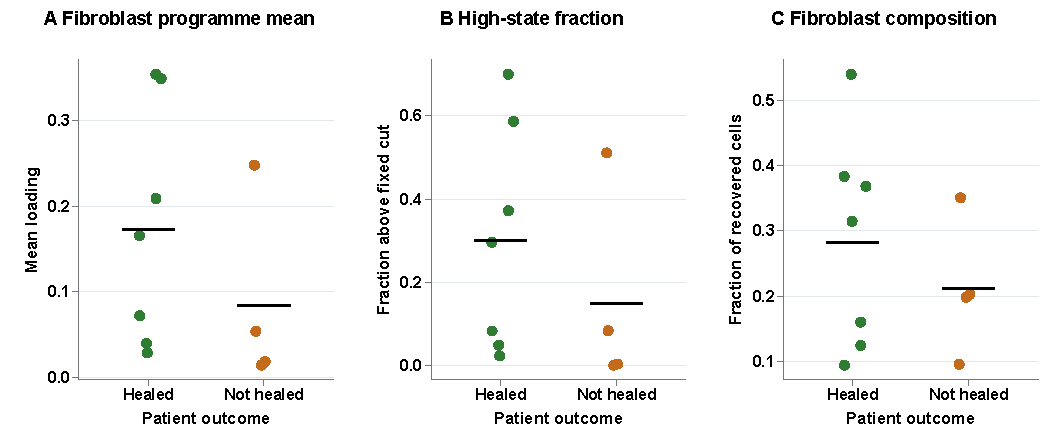
\includegraphics[width=180mm]{../figure5_patient_readouts.pdf}\par\vspace{3mm}
{\fontsize{9}{11.5}\selectfont Patient-unit evaluation of three distinct tissue readouts. In A--C, each point represents one of 7 healed or 4 non-healed DFU patients; horizontal bars show group means. Repeated specimens are pooled within patient using the relevant cell counts, with no outcome-based change to the model or threshold. (A) Mean loading among fibroblasts: healed-minus-non-healed difference 0.0892, exact permutation p=0.3121. (B) Fraction of fibroblasts above the fixed threshold: difference 0.1514, p=0.3697. (C) Fibroblast fraction among all recovered cells: difference 0.0708, p=0.4697. All 330 patient-label allocations enter each two-sided test without add-one correction; BH adjustment over the three tests gives q=0.4697 for each. Patient-bootstrap intervals and weighting sensitivities are reported separately. Points are independent patient summaries for the outcome comparison, not cell-level replicates. (D) High-state patient contrast across eight fixed cuts and the original midpoint; the full-support patient distribution statistic gives p=0.1848 over all 330 label allocations. (E) Mean and full range of contrasts over 250 draws of 100 fibroblasts per specimen, averaging specimens equally within patient. (F) Mean and full range over all eight choices of one specimen per patient. Ranges in E and F are sensitivity ranges, not confidence intervals.\par}
\newpage
{\fontsize{13}{16}\selectfont\bfseries Figure 6}\par\vspace{3mm}
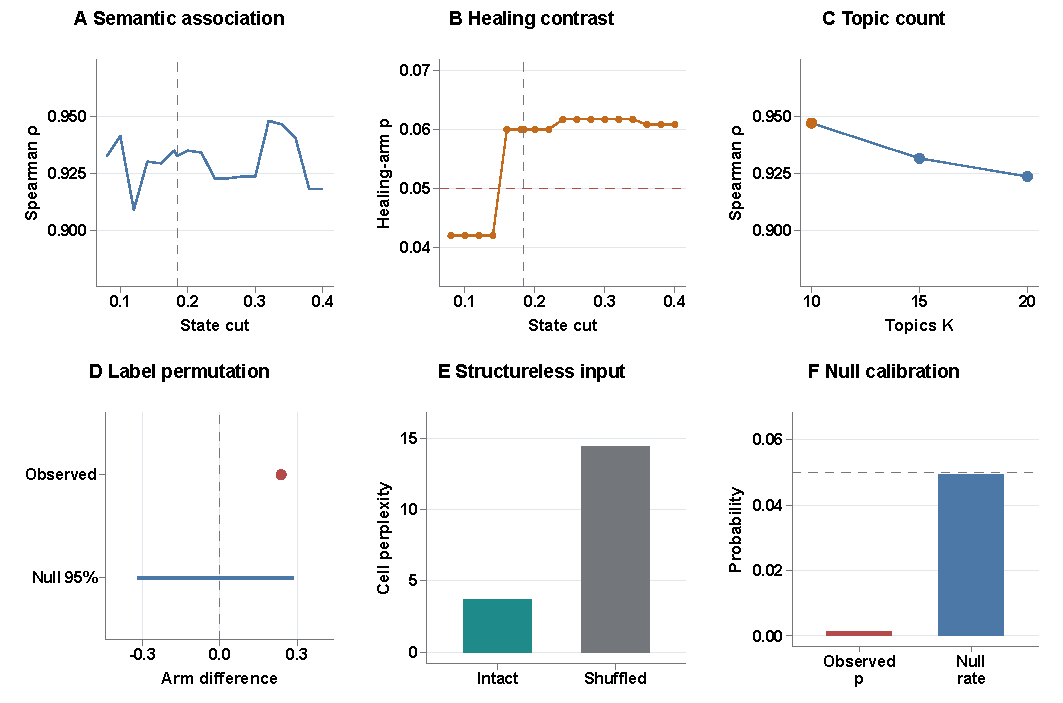
\includegraphics[width=180mm]{../figure6_sensitivity_negative_controls.pdf}\par\vspace{3mm}
{\fontsize{9}{11.5}\selectfont Threshold, capacity and negative-control analyses. (A) Each point gives the Spearman correlation between mean fibroblast loading and high-state fraction across 25 discovery specimens at one of 18 cuts from 0.08 to 0.40. The vertical dashed line marks the pooled fitted cut, 0.1842958. (B) Each point gives the two-sided Mann--Whitney healing-arm p value for 9 healing versus 5 non-healing specimens at the same cuts. The vertical line marks the fitted cut and the horizontal line marks p=0.05; 4 of 18 values fall below that level. (C) Correlations for K=10, 15 and 20 after tracking the TIMP1-carrying topic; orange marks K=10, where the highest fraction is no longer in healthy skin. (D) The observed high-state-fraction arm difference is compared with the central 95\% of 2,002 DFU-only label allocations (p=0.1199); healthy controls were excluded before allocation. (E) Raw-count gene-wise shuffling of 6,000 cells raises mean cell perplexity from 3.44 to 11.23 out of 15 and lowers the mean HHI from 0.574 to 0.147. The shuffle is a co-expression-structure control because row-wise library-size and detection-rate variation also narrow. (F) The anatomical sample-level control compares 33 foot and 11 forearm specimens: observed p=0.0015, with 5.0\% of permuted comparisons below 0.05. This calibration is distinct from the paired 10-patient anatomy analysis and does not establish pipeline-wide error control.\par}
\newpage
{\fontsize{13}{16}\selectfont\bfseries Figure 7}\par\vspace{3mm}
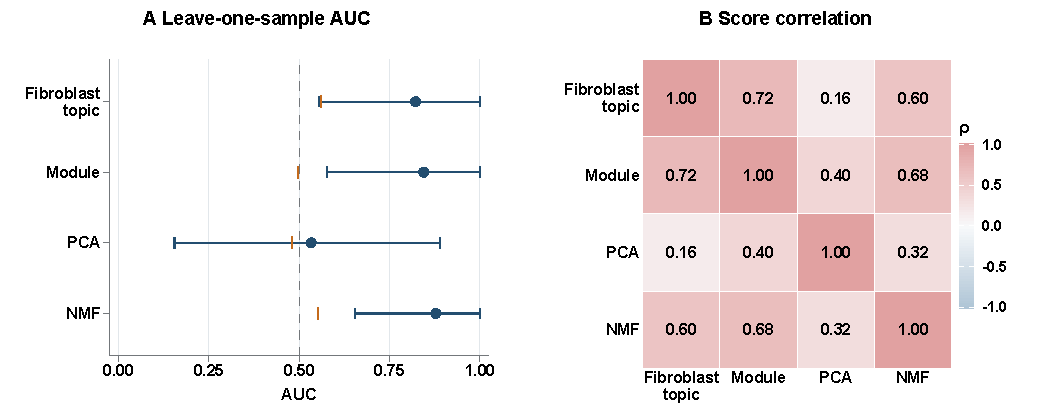
\includegraphics[width=180mm]{../figure7_representation_inference.pdf}\par\vspace{3mm}
{\fontsize{9}{11.5}\selectfont Historical specimen-unit scoring diagnostics in 14 DFU specimens (9 healing, 5 non-healing). (A) Points are leave-one-sample-out areas under the ROC curve (AUCs); horizontal bars are percentile 95\% intervals from 4,000 arm-stratified bootstrap draws of fixed out-of-fold scores, with common resampling indices across methods. Orange ticks mark the procedure-specific permutation-null means after rerunning outcome-dependent fitting and orientation. The dashed line at AUC=0.5 is a visual reference, not the fitted permutation null. Fibroblast topic denotes the frozen all-cell mean, Module the specified fibro-inflammatory score, PCA principal component analysis, and NMF nonnegative matrix factorization. Raw PCA/NMF coordinates can differ across fitted folds, so neither their pooled AUCs nor the displayed bootstrap contrasts support a representation ranking. (B) Cells contain Spearman correlations of these 14 specimen-level readouts; the colour scale and printed values encode the same statistic. Repeated patients and cross-fold comparability limit these historical diagnostics.\par}
\newpage
{\fontsize{13}{16}\selectfont\bfseries Figure 8}\par\vspace{3mm}
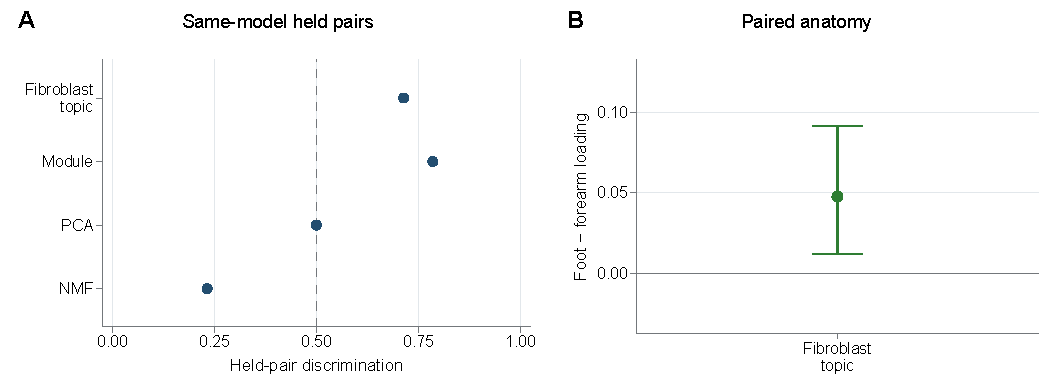
\includegraphics[width=180mm]{../figure8_patient_unit_anatomy.pdf}\par\vspace{3mm}
{\fontsize{9}{11.5}\selectfont Same-model patient-pair discrimination and paired anatomical sensitivity. (A) Each point averages 28 held healing/non-healing pair comparisons from 7 healing and 4 non-healing patients, after cell-count-weighted collapse of repeated specimens. A scoring function fitted to the other nine patients scores both held patients; an equal score earns half credit. The dashed line marks 0.5. Fibroblast topic, Module, PCA and NMF denote the frozen topic mean, fibro-inflammatory module, principal component and nonnegative matrix factorization readouts. NMF component selection uses a training-SD-standardized contrast. No interval is shown: the 28 pairs share patients and are not independent replicates. (B) The point is the mean all-cell fibroblast-associated topic loading difference, foot minus forearm, across 10 paired patients; the bar is a 4,000-draw paired-patient bootstrap 95\% interval and the horizontal line is zero. The exhaustive sign-flip test with add-one correction gives p=0.0107 and Benjamini--Hochberg q=0.0402 across 15 topics. Both panels use the discovery source and are not independent clinical validation.\par}
\newpage
{\fontsize{13}{16}\selectfont\bfseries Figure 9}\par\vspace{3mm}
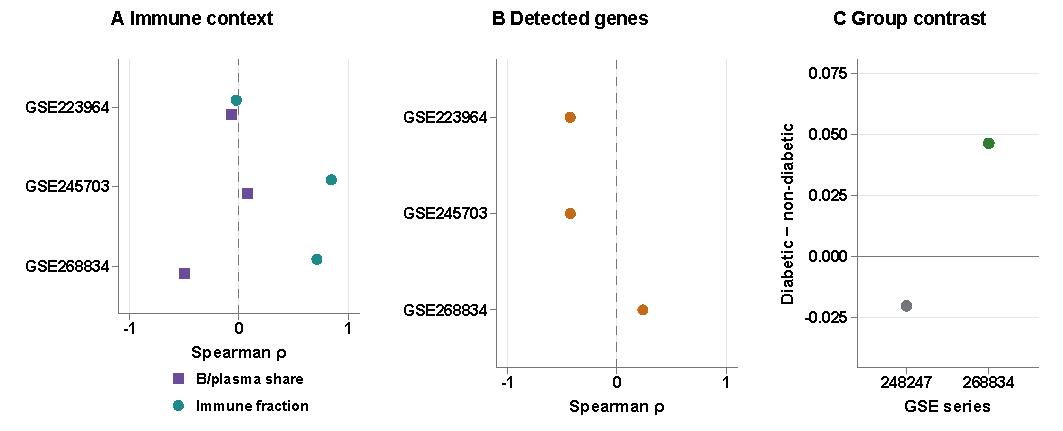
\includegraphics[width=180mm]{../figure9_external_construct_audit.pdf}\par\vspace{3mm}
{\fontsize{9}{11.5}\selectfont Frozen external projections under mutually exclusive lineage gates. Correlations use 8 GSE223964, 12 GSE245703 and 8 GSE268834 specimens. (A) Each point is a cohort-level Spearman correlation between the sample mean fibroblast-associated topic loading within fibroblasts and either immune fraction among all QC cells (teal circles) or B/plasma share within immune cells (purple squares). (B) Orange points correlate the same topic mean with median detected genes per cell. The vertical dashed lines in A and B mark zero. (C) Points show diabetic-minus-non-diabetic differences in the sample fibroblast mean: +0.0464 in GSE268834 (descriptive permutation p=0.2812) and −0.0204 in GSE248247 (p=1.0). GSE248247 contains one specimen per group and 358 QC cells, so its correlations are not estimated. No panel displays confidence intervals. These cohorts lack qualifying patient-level healing endpoints and are not pooled for prognosis inference.\par}
\end{document}
